\subsection{问题}
在初始条件 
\[f_j = \left\{ 
\begin{aligned}
  x_j \qquad         &0 \leq x \leq \pi \\
  2 \pi - x_j \qquad &\pi \leq x \leq 2\pi 
\end{aligned}
 \right. \]
 下, 使用Forward-Euler, Lax-Friedrichs, Lax-Wendroff方法
 数值求解 
 \[ u_t = u_x \]

\subsection{准确解}
使用$h = 2 * \pi / 5000, k = h / 2$ Lax-Wendroff 方法的数值模拟结果作为精确解.


\subsection{Forward-Euler}
$h = 2 \pi / 10, 2 \pi / 100, k = h / 2$的结果都explosion, 如下图

\begin{figure}[!h]
  \centering
  \subfigure[$h = 2\pi / 10$]{
  \begin{minipage}[t]{0.5\linewidth}
  \centering
  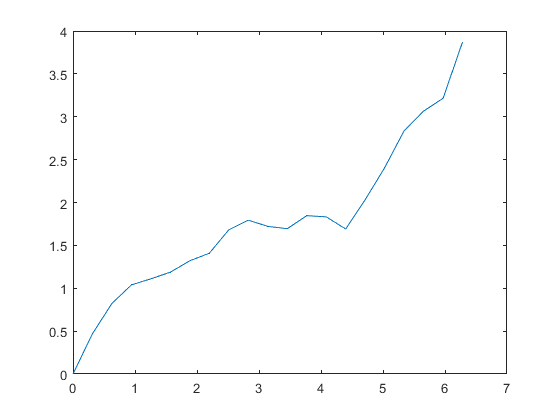
\includegraphics[height=2.5in, width=2.5in]{fig/forwardEulerPeriodTest1LiError.png}
  %\caption{fig1}
  \end{minipage}%
  }%
  \subfigure[$h = 2\pi / 100$]{
  \begin{minipage}[t]{0.5\linewidth}
  \centering
  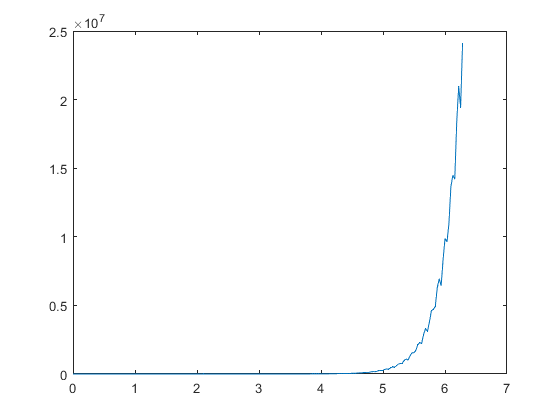
\includegraphics[height=2.5in, width=2.5in]{fig/forwardEulerPeriodTest2LiError.png}
  %\caption{fig2}
  \end{minipage}%
  }%
\end{figure}

\subsection{ Lax-Friedrichs 和 Lax-Wendroff}
结果没有explosion, $h$更小时误差收敛到更小, Lax-Wendroff效果更好一点.
\begin{figure}[!h]
  \centering
  \subfigure[Lax-Friedrichs]{
  \begin{minipage}[t]{0.5\linewidth}
  \centering
  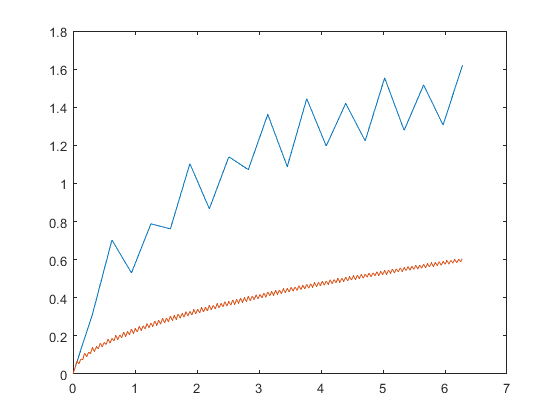
\includegraphics[height=2.5in, width=2.5in]{fig/laxFriedrichsPeriodTestError.png}
  %\caption{fig1}
  \end{minipage}%
  }%
  \subfigure[Lax-Wendroff]{
  \begin{minipage}[t]{0.5\linewidth}
  \centering
  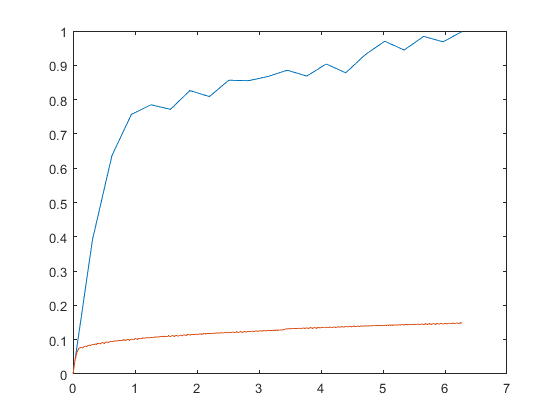
\includegraphics[height=2.5in, width=2.5in]{fig/laxWendroffPeriodTestLiError.png}
  %\caption{fig2}
  \end{minipage}%
  }%
\end{figure}